% Define the introduction
\section{Introduction}

\subsection{Context}

\begin{frame}
    \frametitle{Overview of Computer Science and its Evolution}

    \includegraphics[width=\textwidth]{../images/1-introduction/timeline.pdf}

    \note<1>{
        \begin{itemize}
            \item ``Computer Science is the study of computation and information.''~\cite{university_of_york_what_nodate}
            \item Evolution of Computer Science: From traditional programming to advanced Machine Learning (ML) and Deep Learning (DL) techniques.
            \item Importance of Big Data and Parallel Computing: Catalysts for advancements in ML and DL.
            \item Role of Deep Learning: Automated feature extraction, particularly effective in tasks like image and audio processing.
            \item Significance of Generative Models: Creating synthetic data for various applications.
        \end{itemize}
    }

    \note<2>{
        \begin{enumerate}
            \item \textbf{1646 - Birth of Leibniz:}
                  \begin{itemize}
                      \item Gottfried Wilhelm Leibniz, the founder of computer science, is born.
                  \end{itemize}

            \item \textbf{1958 - Birth of Modern AI:}
                  \begin{itemize}
                      \item F. Rosenblatt proposes three fundamental questions leading to the development of the perceptron.
                  \end{itemize}

            \item \textbf{1960s - Perceptron Convergence:}
                  \begin{itemize}
                      \item Intensive work on convergence algorithms for the perceptron.
                  \end{itemize}

            \item \textbf{1969 - First Winter of AI:}
                  \begin{itemize}
                      \item Minksy and Papert demonstrate the limitations of perceptrons, leading to a slowdown in AI research.
                      \item This led to the first AI winter.
                  \end{itemize}
        \end{enumerate}
    }

    \note<3>{
        \begin{enumerate}
            \item \textbf{1980s - Emergence of Multilayer Neural Networks:}
                  \begin{itemize}
                      \item Studies on learning under multilayer neural networks.
                  \end{itemize}

            \item \textbf{1986 - Backpropagation:}
                  \begin{itemize}
                      \item Rumelhart et al. describe backpropagation, a key learning procedure for neural networks.
                  \end{itemize}

            \item \textbf{1990s - Second Winter of AI:}
                  \begin{itemize}
                      \item Decreased investments in ML due to lack of real successes.
                  \end{itemize}

            \item \textbf{Turn of the Millennium - Resurgence of ML:}
                  \begin{itemize}
                      \item Emergence of three trends: Big Data, reduced cost of parallel computing, and interest in Deep Neural Networks (DNN).
                  \end{itemize}
        \end{enumerate}
    }

    \note<4>{
        \begin{enumerate}
            \item \textbf{2010s - DL in Everyday Applications:}
                  \begin{itemize}
                      \item DL becomes integral for various computer-made tasks, including text translation, recommender systems, and more.
                      \item Introduction of generative models and their applications in image and text generation.
                  \end{itemize}

            \item \textbf{2020s - Decade of Generative Applications:}
                  \begin{itemize}
                      \item Rise of generative models in various applications, including audio processing.
                  \end{itemize}
        \end{enumerate}
    }
\end{frame}


\subsection{Background}

\begin{frame}
    \frametitle{Digital Audio Processing}

    \begin{center}
        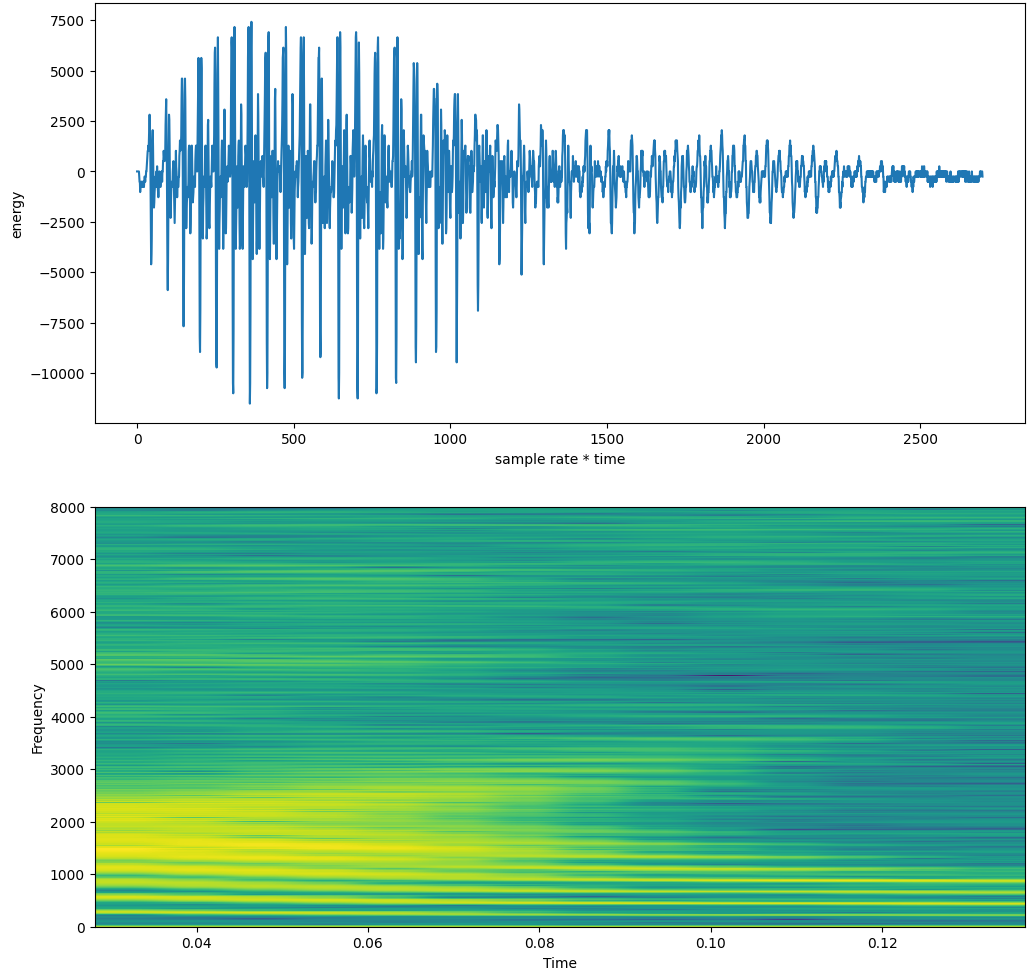
\includegraphics[width=\textwidth, height=0.8\textheight, keepaspectratio]{images/1-introduction/sound_sample.png}
    \end{center}

    \note<1>{
        \begin{itemize}
            \item Sound can be discretized by sampling at a specific time rate, known as the sampling rate.
            \item Sampling rate impacts the accuracy of the signal, with the standard value being 44,100 Hz.
            \item Sound can be represented digitally as an array, enabling reconstruction by a computer.
        \end{itemize}

        \textbf{Short-Time Fourier Transform (STFT):}
        \begin{itemize}
            \item The STFT allows the analysis of the frequency content of a signal over time.
            \item It computes the Fourier Transform of the input signal within windowed time intervals.
            \item The resulting time-frequency representation is used to generate spectrograms.
        \end{itemize}
    }

    \note<2>{
        \textbf{Spectrograms and Machine Learning:}
        \begin{itemize}
            \item Spectrograms represent sound as a time-frequency image, enabling analysis and processing.
            \item Convolutional Neural Networks (CNNs) can be used for sound analysis, but filter shapes and convolution axes require careful consideration.
        \end{itemize}

        \textbf{Soundscapes:}
        \begin{itemize}
            \item Soundscapes are complex mixes of sounds heard in everyday life.
            \item They encompass natural, human-made, and cultural sounds, creating immersive auditory environments.
            \item Generating soundscapes with machine learning is challenging due to their lack of specific structure.
        \end{itemize}
    }
\end{frame}

\begin{frame}
    \frametitle{Foundations for Enhancing Generative Models for Audio}

    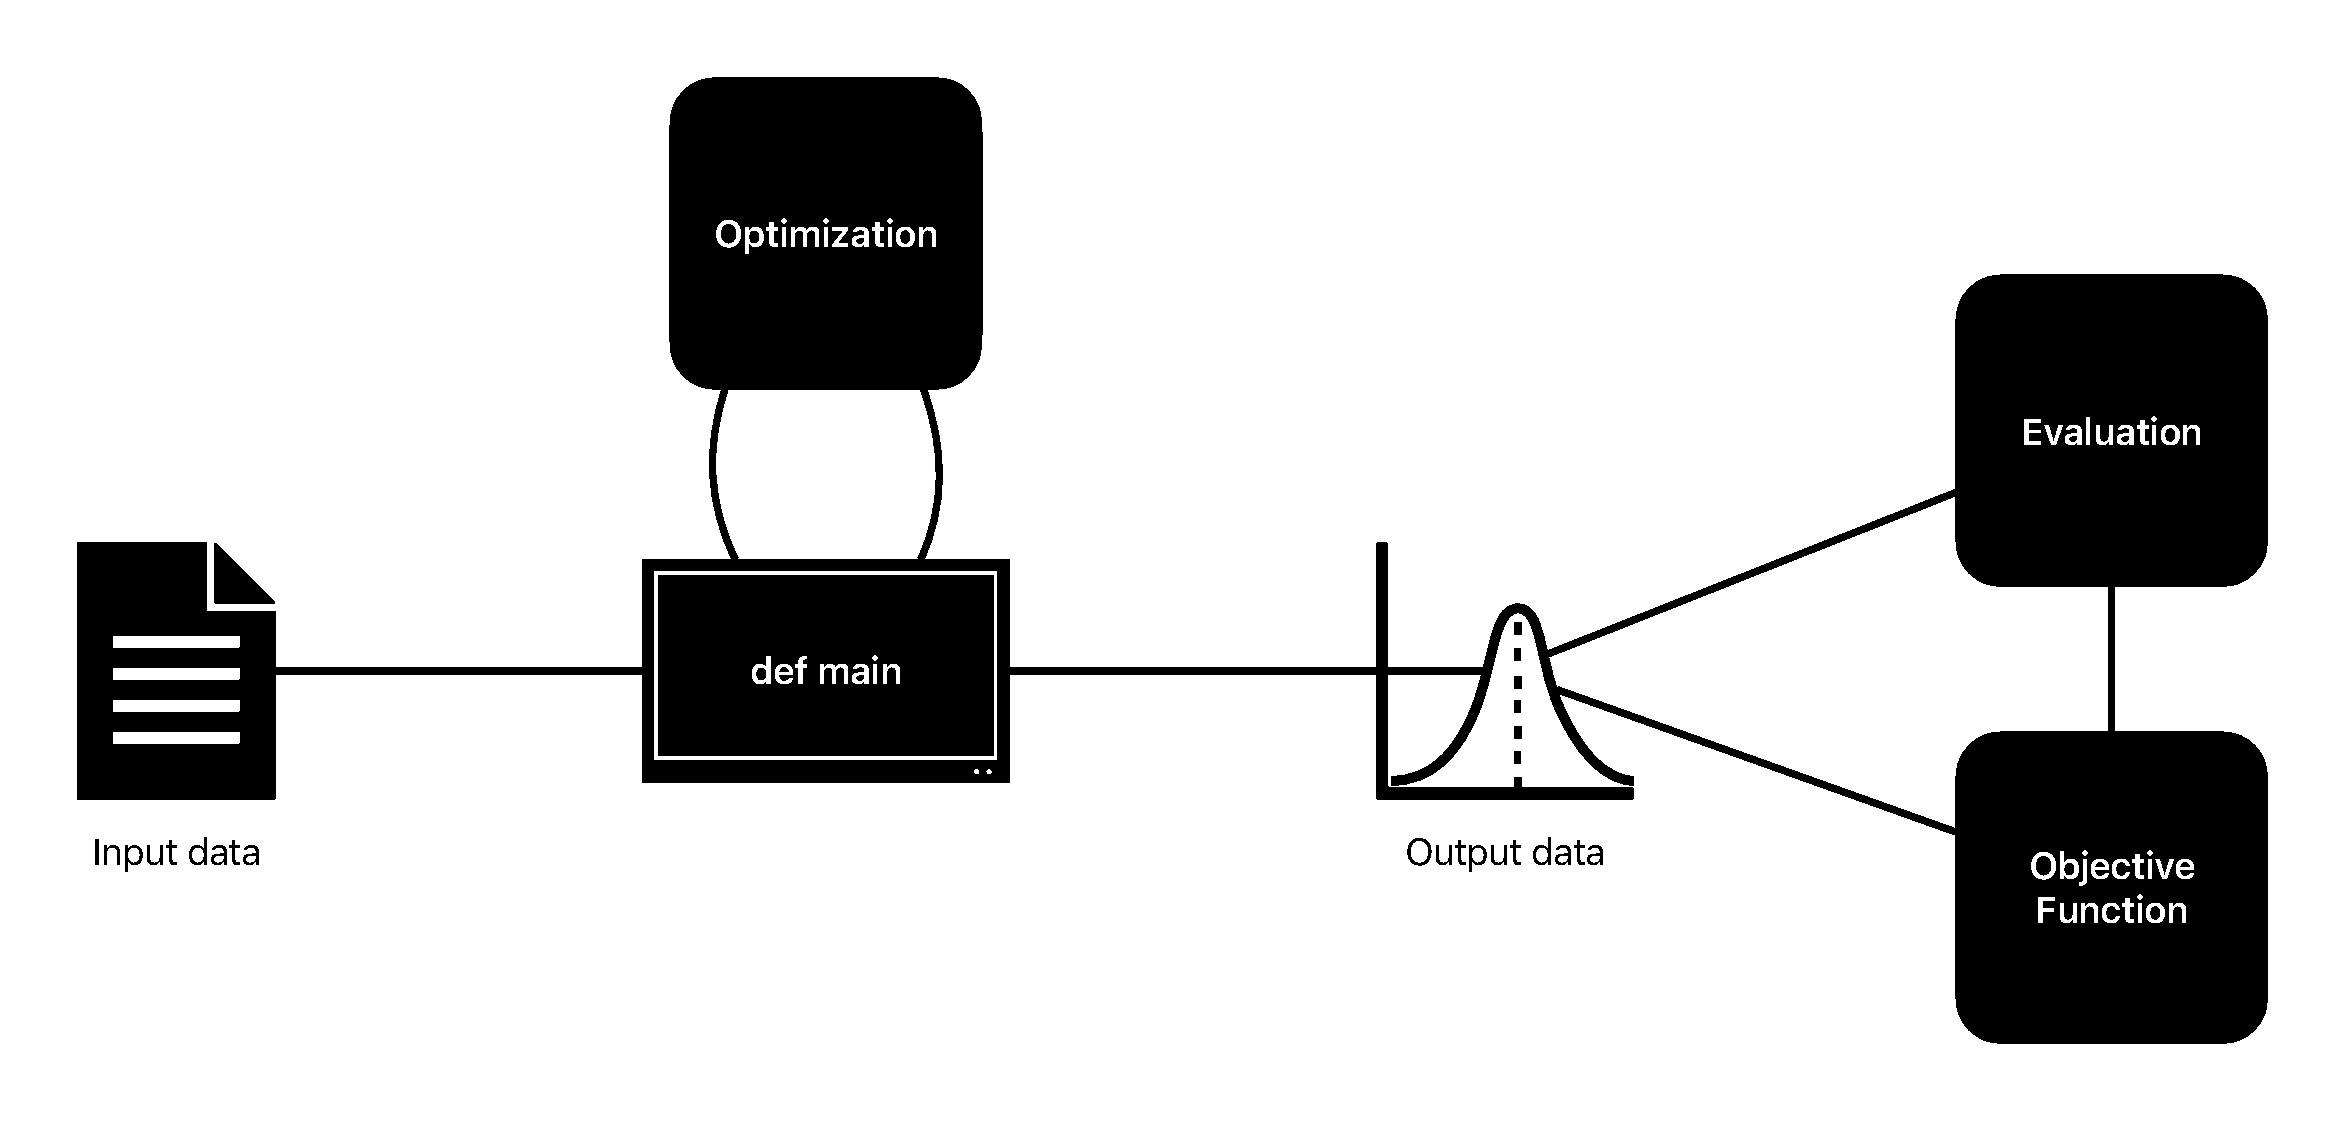
\includegraphics[width=\textwidth]{images/1-introduction/Problem-Definition.pdf}

    \note{

        \begin{itemize}
            \item \textbf{Data Augmentation:} Applying transformations to the original data to increase its size and diversity. This can improve the generalization and robustness of the generative models and reduce the risk of overfitting.
            \item \textbf{Data Embedding:} Converting data into numerical representations that capture its essential features and characteristics.
            \item \textbf{Optimization:} Finding the optimal parameters of the generative model that minimize a predefined loss function. This can be done using various optimization algorithms such as Gradient Descent, Adam, or RMSProp.
            \item \textbf{Evaluation Metrics:} Methods used to measure the quality and diversity of the generated sounds. They provide a way to compare different generative models and assess their strengths and weaknesses.
            \item \textbf{Objective Function:} A function that defines the goal of the generative model and quantifies its performance.
        \end{itemize}
    }

\end{frame}


\begin{frame}
    \frametitle{Deep Learning Frameworks}

    \begin{figure}[ht]
        \centering
        
\includegraphics[width=0.2\textwidth]{images/1-introduction/tensorflow.png}\hspace{1cm}
        
\includegraphics[width=0.2\textwidth]{images/1-introduction/pytorch.png}\hspace{1cm}
        
\includegraphics[width=0.2\textwidth]{images/1-introduction/keras.png}
    \end{figure}

    \note{
        \begin{itemize}
            \item TensorFlow: offers a comprehensive ecosystem for building and deploying machine learning models, including support for audio-related tasks. TensorFlow provides a static computation graph and is known for its scalability and performance.

            \item PyTorch: has gained popularity due to its ease of use and dynamic computation graph, which allows for more flexibility and intuitive programming. PyTorch offers a user-friendly API and is known for its flexibility and support for various applications.

            \item Keras: Keras is a high-level deep learning library that runs on top of TensorFlow. It provides a user-friendly interface for building and training neural network models. Keras simplifies the creation of neural networks by abstracting away many low-level details, making it a popular choice for beginners.

        \end{itemize}

        In this thesis, we have selected PyTorch as the deep learning framework of choice due to its flexibility, ease of use, and optimal performance for our specific tasks.
    }
\end{frame}


\begin{frame}
    \frametitle{Generative Deep Learning Architectures}
    \begin{itemize}
        \item Deep autoregressive networks (DARNs)
        \item Variational autoencoders (VAEs)
        \item Generative adversarial networks (GANs)
        \item Normalizing flows
        \item Diffusion models
        \item Transformers
        \item Vector quantized variational autoencoders (VQ-VAEs)
        \item Multi-scale vector quantized variational autoencoders (MS-VQ-VAEs)
    \end{itemize}

    \note<1>{
        \begin{itemize}
            \item Generative deep learning architectures are designed to generate new and diverse data samples from a learned distribution.
            \item They learn to estimate the underlying probability distribution of the data by minimizing some distance or loss function between the model and the actual distribution.
            \item They have been applied to various tasks, such as image synthesis, text generation, and audio synthesis.
        \end{itemize}
    }
    
    \note<2>{
        \begin{itemize}
            \item In this thesis, we focus on some of the most popular and influential generative deep learning architectures, such as:
                  \begin{itemize}
                      \item Deep autoregressive networks (DARNs)
                      \item Variational autoencoders (VAEs)
                      \item Generative adversarial networks (GANs)
                      \item Normalizing flows
                      \item Diffusion models
                      \item Transformers
                      \item Vector quantized variational autoencoders (VQ-VAEs)
                      \item Multi-scale vector quantized variational autoencoders (MS-VQ-VAEs)
                  \end{itemize}
        \end{itemize}
    }
\end{frame}

\subsection{Motivation}

\begin{frame}{Motivation}
    \begin{enumerate}
        \item \textbf{Revolutionizing Sound Generation}
        \item \textbf{Need for Further Research}
        \item \textbf{Impact and Contribution}
    \end{enumerate}

    \note{
        \begin{enumerate}
            \item \textbf{Revolutionizing Sound Generation}
                  \begin{itemize}
                      \item Integration of ML transforms sound creation and experience.
                      \item Opens creative avenues for artists, impacts industries like film, gaming, VR.
                  \end{itemize}
            \item \textbf{Need for Further Research}
                  \begin{itemize}
                      \item Urgency for studies in sound generation technologies.
                      \item This dissertation contributes significantly, offering resources for exploration.
                  \end{itemize}
            \item \textbf{Impact and Contribution}
                  \begin{itemize}
                      \item Reshaping human potential in sound creation through digital technologies.
                      \item Valuable resource for audio processing professionals, guiding future endeavors.
                  \end{itemize}
        \end{enumerate}
    }
\end{frame}

\subsection{Research objectives}

\begin{frame}{Research Objectives}
    \begin{enumerate}
        \item Make a study of the current state-of-the-art deep learning architectures, focusing on generative ones.
        \item Examine prior algorithms that can process sound for augmentation, feature extraction, or other purposes.
        \item Make a study of the current state-of-the-art architectures used to develop sounds artificially.
        \item Develop end-to-end systems that can synthesize sound from any given text input, while accounting for hardware constraints and ensuring reliable performance.
        \item Evaluate the systems’ ability to generate a sound from the given textual input accurately.
    \end{enumerate}
\end{frame}